%\documentclass[a4paper]{article}
\documentclass[a4paper,twocolumn]{article}
%\documentclass[a4paper,landscape,twocolumn]{article}
%\documentclass[a4paper]{memoir}
\usepackage[utf8]{inputenc}
\usepackage[spanish, es-tabla, es-nodecimaldot]{babel}
%\usepackage[english]{babel}
\usepackage{amsmath}  %permite usar \text{} en el entorno Matemática
\usepackage{amssymb} % para el de números reales
%\usepackage{fancyhdr} %para encabezados y pies de página lindos
%\usepackage{lastpage} %para poder referenciar el número de la última página
\usepackage{graphicx} %para insertar gráficos
\usepackage{float} %para que funcione el H de la posición de las figuras
%\usepackage{chngpage} %para cambiar márgenes temporalmente. Por ejemplo tabla o figura un poco más grande que el text width
%\usepackage[format=plain, indention=0cm, font=small, labelfont=bf, labelsep=period, textfont=sl]{caption} %tuneado del caption de las figuras
\usepackage{mathtools} % para usar dcases, la versión displayMath de cases (funciones partidas)
\usepackage{enumerate} %para personalizar los enumeradores
\usepackage{framed} %para poner párrafos adentro de un caja con marco
%\usepackage{fullpage}
%\usepackage[cm]{fullpage}
\usepackage{array}
\usepackage{hyperref}
\usepackage{epigraph}
\usepackage{wrapfig} %para poner tablas o figuras con texto alrededor.
\usepackage{bbm} %para la función indicadora
\usepackage{enumitem} %para poner títulos y seguir la numeración
\usepackage{multicol}
\usepackage{enumitem}
\usepackage[font=small,labelfont=bf, labelsep=period, width=.45\textwidth]{caption} %tuneado de captions en figuras
\usepackage[nottoc]{tocbibind} %incluir referencias en el toc (table of contents, i.e. índice)



\newcolumntype{x}[1]{>{\centering\arraybackslash\hspace{0pt}}p{#1}}

%\setlength{\columnseprule}{0.5pt}
\setlength{\columnsep}{1cm}

\setlength{\epigraphwidth}{.38\textwidth}
%\setlength{\epigraphwidth}{0.7\textwidth}

\DeclareMathOperator*{\argmax}{argmax} % thin space, limits underneath in displays


%\usepackage{amssymb,amsmath,amsthm,latexsym,epsfig,euscript,multicol}
%\usepackage{enumitem}
%\usepackage[utf8x]{inputenc}

% Caracteres especiales
%\def\A{\mathbb{A}}
\def\C{\mathbb{C}}
\def \N{\mathbb{N}}
%\def \P{\mathbb{P}}
%\def \Q{\mathbb{Q}}
\def \R{\mathbb{R}}
%\def \Z{\mathbb{Z}}
\def \sen{\textrm{sen}}

%\theoremstyle{definition}
%\newtheorem{ejer}{Ejercicio}
%\newcommand{\bej}{\begin{ejer}}
%	\newcommand{\fej}{\end{ejer}}

%\def\dt{\Delta t}
%\def\dx{\Delta x}

\def\eps{\varepsilon}
%\def\wt{$\widetilde{a}$}



\title{TP AID 2021 cuat. 1\\ Análisis de asociación entre personalidad y consumo de drogas }
\author{Alumno: G. Sebastián Pedersen {\small (sebasped (at) gmail (dot) com)}\\ Docente: Débora Chan }

\date{}




\renewcommand{\arraystretch}{1.3}  %para que las celdas de las tablas sean un poco más altas y entre bien el Q moño.




\begin{document}
%\pagestyle{headings}
%\markright{John Smith\hfill On page styles\hfill}

	
\maketitle

\tableofcontents	
	%\begin{abstract}
	%	Se propone un primer modelo, clásico y sencillo, que intenta capturar la idea de cuándo un estudiante entra en riesgo de deserción de una materia.
	%\end{abstract}
	%\tableofcontents



\section{Introducción}
Los problemas de detectar o evaluar el riesgo de consumo y abuso de drogas, en especial ilegales, son de considerable importancia actual. En el presente trabajo se aborda el análisis de la asociación entre personalidad y consumo de drogas, haciendo énfasis en ilegales, y usando datos recolectados mediante encuestas anónimas, las cuales registraron  datos de personas sobre la personalidad (cinco scores del NEO-FFI-R, una variante del conocido Five Factor Model; la impulsividad mediante el BIS-11 y la búsqueda de sensaciones mediante el ImpSS) y el consumo de diversas drogas legales e ilegales, además de rango etario, sexo, nivel de educación, nacionalidad y etnia. 

%En el análisis se utilizaron diversas técnicas de clasificación supervisada y no supervisada, mostrándose para cada uno de los dos casos la técnica más efectiva, siempre en dirección a responder el problema al principio formulado. 


\section{Datos y prepocesado}

\subsection{Datos crudos}
Para el análisis se utilizaron datos provenientes de encuestas anónimas. La base de datos está disponible online (ver \cite{dataset}) y consta de 1885 observaciones. En cada encuesta, es decir cada persona u observación, se registraron las siguientes variables, divididas simplemente por mayor claridad en tres grupos:
\begin{enumerate}[label=\roman*)]
	\item Variables demográficas:
	\begin{itemize}%[label=\roman*)]
		\item Edad: 18-24; 25-34; 35-44; 45-54; 55-64 y 65 o más.
		\item Sexo: femenino; masculino.
		\item Educación:
		\begin{enumerate}[label=\arabic*)]
			\item Dejó la escuela antes de los 16 años.
			\item Dejó la escuela a los 16 años.
			\item Dejó la escuela a los 17 años.
			\item Dejó la escuela a los 18 años.
			\item Terminó la escuela o cursó algo de terciario o universitario, pero no tiene algún título.
			\item Tiene título profesional.
			\item Tiene título universitario.
			\item Tiene título de maestría.
			\item Tiene título de doctorado.
		\end{enumerate}
		\item País de residencia.
		\item Etnia.
	\end{itemize}
	\item Variables sobre la personalidad (\mbox{NEO-FFI-R} ver \cite{neoffir}, BIS-11 ver \cite{bis11}, ImpSS ver \cite{impss}):
	\begin{itemize}%[resume]
		\item Nscore: score sobre neurotismo, medido por \mbox{NEO-FFI-R}.
		\item Escore: score sobre extraversión, medido por \mbox{NEO-FFI-R}.
		\item Oscore: score la apertura a experimentar, medido por \mbox{NEO-FFI-R}.
		\item Ascore: score sobre la complacencia, medido por \mbox{NEO-FFI-R}.
		\item Cscore: score sobre la conciencia, medido por \mbox{NEO-FFI-R}.
		\item Impulsive: score sobre la impulsividad, medido por \mbox{BIS-11}.
		\item SS: score sobre la búsqueda de sensaciones, medido por \mbox{ImpSS}.
	\end{itemize}
	\item Variables sobre el consumo de drogas, medidas con las siguientes categorías:
	\begin{enumerate}[label=\arabic*)]
		\item CL0: nunca consumió.
		\item CL1: consumió hace más de una década.
		\item CL2: consumió en la última década.
		\item CL3: consumió en el último año.
		\item CL4: consumió en el último mes.
		\item CL5: consumió en la última semana.
		\item CL6: consumió en el último día.
	\end{enumerate}
	Las variables en sí mismas son las siguientes:
	\begin{itemize}%[resume]
		\item Alcohol.
		\item Amphet: consumo de amfetaminas
		\item Amyl: consumo de amyl nitritos.
		\item Benzos: consumo de benzodiazepina.
		\item Caff: consumo de cafeína.
		\item Cannabis.
		\item Choc: consumo de chocolate.
		\item Coke: consumo de cocaína.
		\item Crack.
		\item Ecstasy: consumo de éxtasis.
		\item Heroin: consumo de heroina.
		\item Ketamine: consumo de ketamina.
		\item Legalh: consumo de \emph{legal highs} (drogas psicoactivas contenidas en diversos químicos).
		\item LSD.
		\item Meth: consumo de metadona.
		\item Mushrooms: consumo de hongos mágicos.
		\item Nicotine.
		\item Semer: droga ficticia.
		\item VSA: consumo de sustancias volátiles.
	\end{itemize}
\end{enumerate} 



\subsection{Preprocesado}
Se identificó que tanto la variable país de residencia como la variable etnia, estaban muy concentradas en pocas categorías. País de residencia, además de estar concentrada en unos pocos países (6 países y una categoría otros), el casi 85\% de los datos corresponden a UK o USA. Por su parte etnia está concentrada en algo más del 91\% en la raza blanca. Por lo tanto se decidió excluir estas variables del análisis, pues no hay una suficiente diversidad y adecuada distribución como para que tenga sentido considerar su influencia sobre la clasificación. También se decidió excluir del análisis la variable sexo por considerarse no adecuada su influencia en la clasificación.

Para decidir el criterio a tener en cuenta a la hora de considerar el consumo de drogas, tanto cuáles drogas como qué umbral de consumo, se realizó un análisis de correspondencia entre todas las drogas y tomando como variable \emph{sí consume la droga} la correspondiente a los niveles CL3, 4, 5 y 6 (es decir consume significa que consumió en el último año o menos).

\begin{figure}[h]
	\centering
	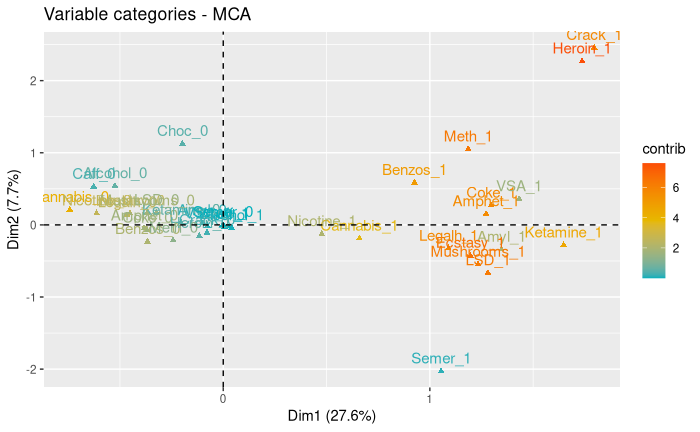
\includegraphics[trim={0.2cm 0.2cm 0.3cm 0.7cm}, clip=true, width=0.48\textwidth]{analCorresp.png}
	\caption{Análisis de correspondencia entre las drogas. La categoría 1 corresponde a haber consumido en el último año o menos.}
	\label{fig:analCorresp}
\end{figure}

En la figura \ref{fig:analCorresp} se observa que el consumo de Semer (\emph{Semer\_1}) está aislado, y como esta droga es ficticia y fue introducida a modo de control, se decidió eliminar las observaciones que indicaron consumo de dicha droga. También se observa que los consumos de nicotina y cannabis están fuertemente asociados, y dado que en los últimos años algunos países han legalizado el consumo de cannabis, se decidió no tenerlas en cuenta (recordemos que el análisis hace énfasis en el consumo de drogas ilegales). Se observa otro grupo que incluye consumo de Meth, Benzos, VSA, Coke, Amphet, Ketamine, Legalh, Amyl, Ecstasy, Mushrooms y LSD. Tomando en cuenta la contribución de cada una de estas drogas y su ilegalidad, se decidió conservar Coke, Ecstasy, LSD y Meth. Se distingue otro grupo, que incluye Crack y Heroin, y se decidió conservar ambas tomando en cuenta ilegalidad y contribución. Finalmente se observa un último grupo, concentrado alrededor de lo más usual, que incluye a todos los no consumos y a los consumos de drogas no ilegales.

Cabe mencionar que se realizaron también análisis de correspondencia tanto exluyendo la droga ficticia Semer, como endureciendo el criterio de \emph{sí consume} a si consumió en el último mes o menos, arrojando resultados similares a los de la figura \ref{fig:analCorresp}, aunque endureciendo el criterio de consumo conllevaba a un mayor desbalanceo de clases. No se consideró como adecuado tanto endurecer aún más el criterio de consumo, como relajarlo más allá del último año.

Finalmente considerando que las variables edad y nivel educativo no iban a ser utilizadas de forma directa en el análisis, pues este se enfoca en la asociación de la personalidad con el consumo de drogas (con énfasis en ilegales), se decidió agrupar aún más estas variables para brindar por un lado mayor interpretabilidad y por el otro una mejor distribución entre sus respectivas categorías (las distribuciones originales se pueden ver de \cite{dataset}). Las nuevas variables se detallan a continuación:

\begin{itemize}
	\item Variable edad nueva: 18-24 (34.11\% de las obs.); 25-34 (25.52\%); 35 o más (40.37\%).
	\item Variable nivel educativo nueva:
	\begin{enumerate}[label=\arabic*)]
		\item Dejó la escuela a los 18 años o antes (13.64\% de las obs.).
		\item Terminó la escuela o cursó algo de terciario o universitario, pero no tiene algún título (26.84\%).
		\item Es un profesional no universitario (14.32\%).
		\item Tiene título universitario o mayor (45.19\%).
	\end{enumerate}
\end{itemize}

Observemos que el nivel educativo está claramente sesgado hacia el nivel mayor. Deberemos tener en cuenta esto a la hora de realizar el análisis y derivar conclusiones.

Resumiendo, y tomando en cuenta los preprocesos antes mencionados, la cantidad de observaciones disminuyó a 1877, quedando balanceadas en 42\% y 58\% entre consume y no consume drogas respectivamente, y las variables finales utilizadas fueron las siguientes:

\begin{itemize}
	\item Edad nueva: 18-24; 25-34 y 35 o más.
%	\item Sexo: femenino; masculino.
	\item Eduación nueva:
	\begin{enumerate}[label=\arabic*)]
		\item Dejó la escuela a los 18 años o antes.
		\item Terminó la escuela o cursó algo de terciario o universitario, pero no tiene algún título.
		\item Es un profesional no universitario.
		\item Tiene título universitario o mayor.
	\end{enumerate}
	\item Nscore: score sobre neurotismo.
	\item Escore: score sobre extraversión.
	\item Oscore: score la apertura a experimentar.
	\item Ascore: score sobre la complacencia.
	\item Cscore: score sobre la conciencia.
	\item Impulsive: score sobre la impulsividad.
	\item SS: score sobre la búsqueda de sensaciones.
	\item Consume: variable que indica si consume o no drogas, siendo que sí consume si es que consumió alguna de las drogas cocaína, crack, éxtasis, heroína, LSD o metadona, en el último año o menos.
\end{itemize}



\section{Análisis exploratorio}
\label{sec:analExp}
Como primera exploración de los datos, de los boxplots de cada score (N, E, O, A y C), de Impulsive y de SS, se observan distribuciones univariadas simétricas y con algunos outliers no severos, considerando tanto cada variable entera como su separación por la variable Consume. En un plano más formal y técnico se comprueban la normalidad univariada de las mencionadas variables tanto mirando los qqplots como realizando el test de Anderson-Darling (con p-valores menores al 2\%).

Ya que el análisis es sobre la asociación entre la personalidad y el consumo de drogas, una interesante primera medida es contrastar la media del grupo de observaciones que sí consumen contra la de los que no consumen, para analizar si existen diferencias e intentar discernir las variables que mejor pueden clasificar los mencionados grupos.

\begin{figure}[h]
	\centering
	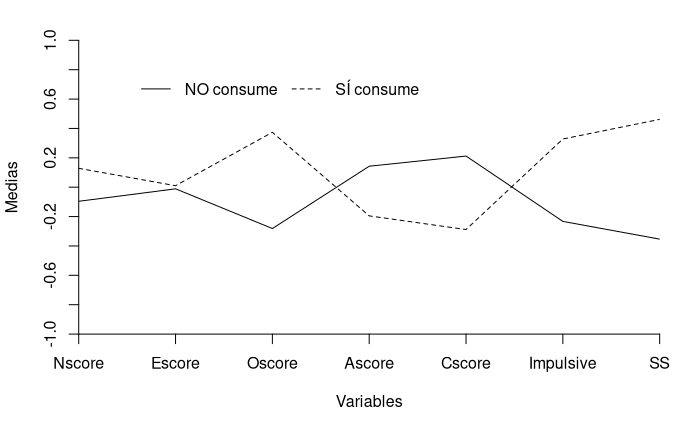
\includegraphics[trim={0.1cm 1.6cm 0.8cm 0.7cm}, clip=true, width=0.48\textwidth]{perfilesMedios.png}
	\caption{Comparación de los perfiles medios multivariados.}
	\label{fig:perfMedios}
\end{figure}

La figura \ref{fig:perfMedios} muestra los perfiles medios de ambos grupos (cabe aclarar que la estimación robusta no presentó diferencias significativas). A simple viste se observa que el grupo que consume tiene, en promedio, más alto el Oscore (apertura a experimentar), la impulsividad y el SS (búsqueda de sensaciones), y más bajo el Ascore (complacencia) y el Cscore (conciencia); observándose lo contrario en el grupo que no consume. Los Nscore (neurotismo) y Escore (extraversión) parecen, al menos en promedio, no influir.

Un resultado análogo se pudo apreciar de los boxplots de las mencionadas variables categorizadas por consume y no consume, arrojando más evidencia sobre la posibilidad de asociar la personalidad al consumo de drogas.

Lamentablemente el test de Shapiro arroja rechazo de la normalidad multivariada, y el M-test de Box rechaza la homocedasticidad entre los dos grupos. Más allá de esto, si de todos modos se aplica el test de Hotelling de comparación de medias multivariadas entre dos grupos (que tiene asidero en su validez asintótica), el resultado es de contundente rechazo de igualdad de medias entre ambos grupos, en la misma línea con lo que se observa en la figura \ref{fig:perfMedios}.

El análisis de componentes principales (ACP) también arroja resultados cualitativamente en la misma línea que los perfiles medios. La figura \ref{fig:pca} muestra el biplot de ACP, cabiendo recalcar que las primeras dos componentes explican algo más del 58\% de la variabilidad (información) total, y que no se observan outliers multivariados. 

\begin{figure}[h]
	\centering
	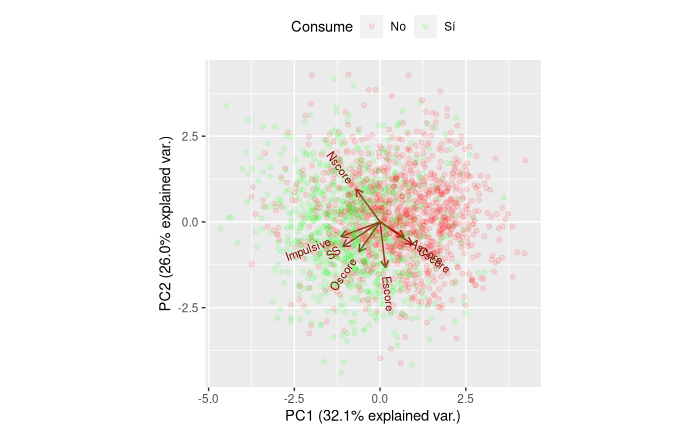
\includegraphics[trim={4cm 0.2cm 2cm 0.5cm}, clip=true, width=0.55\textwidth]{pca.png}
	\caption{Biplot de componentes principales.}
	\label{fig:pca}
\end{figure}

Al igual que para los perfiles medios, la figura \ref{fig:pca} de ACP muestra la misma tendencia: para el grupo que consume altas las variables Oscore (apertura a experimentar), la impulsividad y el SS (búsqueda de sensaciones); y para el grupo que no consume altas las variables Ascore (complacencia) y el Cscore (conciencia); no observándose una influencia clara para las variables Nscore (neurotismo) y Escore (extraversión).

Si se realiza el mismo biplot de la figura \ref{fig:pca} pero discriminando por rango de edad, se distingue una tendencia a no consumir drogas para los mayores de 35 y a consumir en las personas pertenecientes al rango de edad 18-24. Algo similar se observa en el nivel de educación observándose una tendencia a asociar menor consumo con mayor nivel educativo, aunque todavía menos clara que en el caso de la edad y, dada la asimétrica distribución del nivel de educación en los datos, con menor asidero.

\paragraph{Correlaciones entre variables:} mirando la figura \ref{fig:pca} se puede malinterpretar la correlación entre las variables. Desde el dato duro arrojado por el cálculo de las correlaciones, destacamos un 0.62 entre Impulsive y SS; alrededor de un 0.4 entre Nscore y Escore, entre Nscore y Cscore y entre Oscore y SS; con el resto de las correlaciones en el orden de 0.3 o menor.


\section{Clasificación supervisada}
Para estas técnicas de clasificación se separaron los datos en entrenamiento y testeo, en 70\% y 30\% respectivamente, utilizando los datos de entrenamiento para construir el clasificador, y los datos de testeo para testearlo. Además se escalaron los datos de entrenamiento, y se utilizaron estos parámetros de escalado para escalar los datos de testeo. La métrica a maximizar fue siempre el accuracy, es decir el porcentaje de clasificación correcta, tanto positiva como negativa (clasificación positiva es que sí consuma drogas).

Teniendo en cuenta tanto la métrica a maximizar como que no se satisfacen los supuestos de normalidad multivariada ni homocedasticidad, como ya mencionamos en la sección \ref*{sec:analExp}, la técnica que mejores resultados arrojó fue la de support vector machine (SVM), clasificando correctamente (accuracy) el 72.5\% de las observaciones para testeo, consiguiendo además una precisión del 76.6\% (detección de falsos positivos) y un recall del 75\% (detección de falsos negativos). La figura \ref{fig:svm} muestra el biplot de clasificación del SVM, es decir el biplot construido por ACP pero con la clasificación del SVM (léase aplicando el clasificador a la totalidad de los datos y no solamente a los de testeo). Si se compara con el biplot de clasificación real de la figura \ref{fig:pca} se observa el buen comportamiento de este clasificador.

\begin{figure}[h]
	\centering
	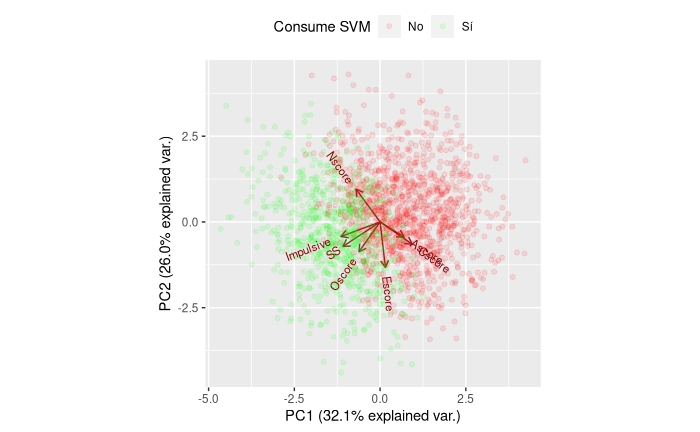
\includegraphics[trim={4cm 0.2cm 2cm 0.5cm}, clip=true, width=0.55\textwidth]{svm.png}
	\caption{Biplot de la clasificación por SVM.}
	\label{fig:svm}
\end{figure}

Resulta también interesante analizar el clasificador del tipo regresión logística. Además de presentar un accuracy similar a SVM, con una precisión algo menor y un recall algo mayor, lo interesante de este clasificador radica en analizar sus coeficientes, pues los mayores positivos están en las variables SS y Oscore, los mayores negativos en las variables Cscore y Ascore, y los relativamente más cercanos a cero en las variables Nscore, Escore y Impulsive. Salvo Impulsive, el resto está en directa correlación con lo observado en la comparación de los perfiles medios de la figura \ref{fig:perfMedios} y en lo observado en el ACP de la figura \ref{fig:pca}. Que Impulsive tenga un coeficiente cercano a cero se explica por su alta correlación lineal con SS (0.62 de coef. de corr.).

Dado que SVM y regresión logística arrojaron resultados similares en cuanto a métricas de evaluación (accuracy, precisión y recall) se procedió a analizar las observaciones (todas, como en la figura \ref{fig:svm}) clasificadas de manera distinta entre ambos clasificadores. En cantidad total son pocas, siendo poco más del 5\% (46 mal clasificadas por SVM pero bien por regresión logística, y 53 en el caso contrario, de un total de 1877). Analizando las observaciones donde hubieron diferencias, en ambos casos se detectaron tres grupos predominantes de observaciones: cercanas al promedio, asociadas al Nscore, y asociadas al Escore. Es interesante relacionar esto con la tendencia observada en la figura \ref{fig:pca} la cual resulta razonable interpretar indicando que el Nscore y el Escore no influyen a la hora de asociar la personalidad con el consumo de drogas. Es decir las observaciones donde los clasificadores difieren o bien son cercanas al promedio, o bien están asociadas a variables de la personalidad que parecen no influir respecto al consumo de drogas.

A pesar de no satisfacerse las hipótesis de normalidad multivariada y homocedasticidad, igualmente se entrenó un clasificador del tipo discriminante lineal (LDA), clasificando correctamente (accuracy) un 72\% de los datos de testeo, con una precisión del 79\% y un recall de 73.6\% (todos valores similares al SVM). Algo interesante de este clasificador LDA radica en analizar sus coeficientes, presentando resultados similares a la regresión logística, y por lo tanto avalando una similar interpretación de las variables en cuanto al consumo o no de drogas.

El clasificador del tipo discriminante cuadrático (QDA), que en principio tendría más sentido que el LDA al no necesitar la hipótesis de homocedasticidad, pero entrenado con la misma salvedad que para LDA de no cumplirse normalidad, arrojó una clasificación (accuracy) similar al LDA, pero con una precisión más baja (63.4\%) y un recall más alto (82.7\%). Este clasificador puede ser de utilidad si se desea focalizar la clasificación en evitar los falsos negativos pero manteniendo el accuracy.

Al no cumplirse el supuesto de normalidad, tampoco es más adecuado el clasificador del tipo discriminante robusto (RDA), que de todos modos fue entrenado, arrojando resultados similares al LDA (accuracy del 71.8\%, precisión del 77.6\% y recall del 73.7\%). %Cabe aclarar que el RDA utilizado incluyó tanto el caso lineal como el cuadrático, pues realiza una optimización utilizando una combinación convexa entre ambos 

Cabe mencionar que en todos los casos los clasificadores arrojaron un resultado similar al mostrado para SVM en la figura \ref{fig:svm}, y por lo tanto avalando con mayor evidencia la relación entre variables y consumo o no de drogas antes mencionado para regresión logística y LDA, y también exhibido gráficamente por los perfiles medios de la figura \ref{fig:perfMedios} y por el biplot de ACP de la figura \ref{fig:pca}.

\subsection{Conclusiones}
La clasificación arroja evidencia en favor de asociar el consumo de drogas a las personalidades con alto Oscore (apertura a experimentar), SS (búsqueda de sensaciones) e Impulsive (impulsividad); y a las personalidades con alto Ascore (complacencia) y Cscore (conciencia) con el no consumo de drogas. Es decir hay evidencia para pensar que un test de personalidad contiene variables que arrojan información importante a la hora de intentar detectar a una persona con riesgo de comenzar a o que está consumiendo drogas.

Además esta clasificación arroja evidencia de que el Nscore (neurotismo) y Escore (extraversión) no tienen una clara influencia en el consumo o no de drogas.





\section{Clasificación no supervisada}
Para estas técnicas de clasificación se utilizaron todos los datos prescindiendo de su clasificación original (es decir si consume o no), y también fueron escalados. Recordemos que estas técnicas buscan estructuras o agrupamientos internos de los datos sin conocer ningún tipo de clasificación sobre los mismos. Cabe aclarar que el análisis se realizó asumiendo que no se posee ningún tipo de clasificación de los datos, e intentando discernir tres (potencialmente dos) grupos de variables que sinteticen: tendencia a experimentar, tendencia a ser cautos, y neutrales respecto de estas dos (potencialmente vacío).

La técnica que mejores resultados arrojó fue la de \mbox{k-means}, pues fue la que mejor agrupó a las observaciones respecto a la interpretación individual de las variables. La figura \ref{fig:kmeans} muestra el biplot de agrupamiento arrojado por k-means, es decir el biplot construido por ACP pero con el agrupamiento dado por k-means, en donde se observa un grupo de observaciones con alto Ascore (complacencia) y Cscore (conciencia); y otro grupo con alto Impulsive (impulsividad), SS (búsqueda de sensaciones), Oscore (apertura a experimentar), y en menor medida Nscore (neurotismo). El Escore (extraversión) parece ser neutro. Es decir hay un grupo con una fuerte tendencia a experimentar de manera impulsiva, y otro grupo mucho más complaciente y concienzudo.

%  Si se compara con el biplot de clasificación real de la figura \ref{fig:pca} se observa que \mbox{k-means} logra capturar bastante bien la estructura de las dos clases, aunque dando más peso al Nscore (neurotismo) en el caso de consumo de drogas. De todas formas es claro que se puede interpretar al cluster 1 como los que no consumen, y al cluster 2 como los que sí. 

\begin{figure}[h]
	\centering
	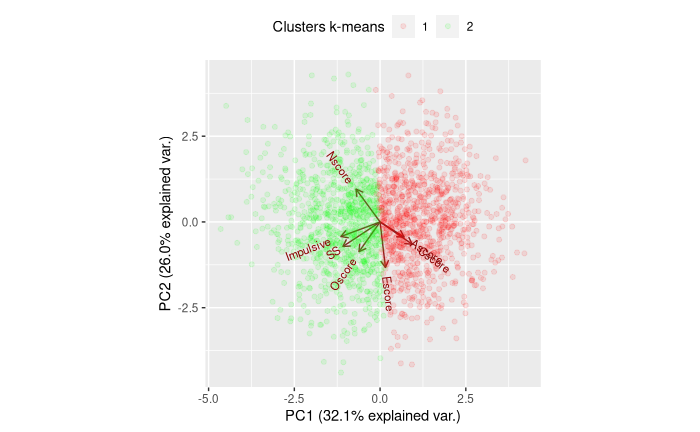
\includegraphics[trim={4cm 0.2cm 2cm 0.5cm}, clip=true, width=0.55\textwidth]{kmeans.png}
	\caption{Biplot del agrupamiento por k-means.}
	\label{fig:kmeans}
\end{figure}

%Interpretando a los clusters de esta manera, \mbox{k-means} clasifica correctamente (accuracy) al 70.3\%, con una precisión del 67.4\% y un recall del 77.9\%. 
Si computamos los perfiles medios de cada cluster, mostrados en la figura \ref{fig:perfMedios_kmeans}, podemos observar un comportamiento coherente con la figura \ref{fig:kmeans}, donde de nuevo se evidencian los mencionados dos grupos provenientes de interpretar los grupos de variables resultantes.

\begin{figure}[h]
	\centering
	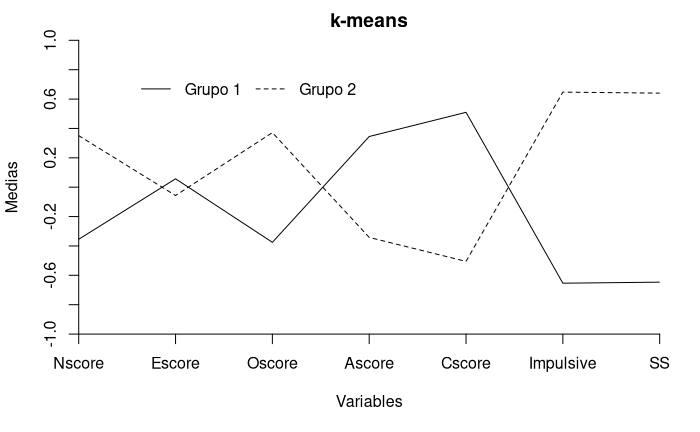
\includegraphics[trim={0.1cm 1.6cm 0.8cm 0.7cm}, clip=true, width=0.48\textwidth]{perfilesMedios_kmeans.png}
	\caption{Comparación de los perfiles medios multivariados de los grupos de k-means.}
	\label{fig:perfMedios_kmeans}
\end{figure}

La técnica de k-means, al no utilizar la clasificación real de los datos, no conoce a priori la cantidad de grupos reales. Por lo tanto es razonable evaluar internamente cuán bien se están separando los datos respecto a la cantidad de agrupamientos. En este sentido se utilizó el coeficiente de Silhouette, el cual arrojó resultados enteramente consistentes con que el mejor agrupamiento es en dos grupos, pues su valor bajó sistemáticamente desde dos hasta quince grupos.

También se probaron técnicas de agrupamiento jerárquico, pero en ningún caso se obtuvieron clasificaciones en grupos razonables de ser interpretados teniendo en cuenta los significados de las variables.

Por último también es interesante mostrar el resultado de k-means agrupando por variables (y no por observaciones como al principio). Tomando en cuenta el objetivo del análisis en este tipo de clasificación, tiene sentido agrupar a las variables en dos o en tres grupos. Para dos grupos el resultado fue:

\begin{itemize}
	\item Grupo 1: Nscore, Oscore, Impusilve, SS.
	\item Grupo 2: Escore, Ascore, Cscore.
\end{itemize}

Si analizamos este agrupamiento respecto a las variables, es razonable interpretar al grupo 1 como las variables que sí influyen a la tendencia a experimentar de manera impulsiva, y al grupo 2 como las variables que no. Para tres grupos el resultado fue:

\begin{itemize}
	\item Grupo 1: Oscore, Impusilve, SS.
	\item Grupo 2: Escore, Ascore, Cscore.
	\item Grupo 3: Nscore.
\end{itemize}

Si nuevamente analizamos este agrupamiento respecto a las variables, es razonable interpretar al grupo 1 como las variables que sí influyen a la tendencia a experimentar de manera impulsiva, al grupo 2 como las que no, y al grupo 3 como las neutras. Si comparamos este agrupamiento con las interpretaciones anteriormente extraídas del agrupamiento por observaciones (figuras \ref{fig:kmeans} y \ref{fig:perfMedios_kmeans}), como única diferencia se observa que hay un intercambio entre Escore y Nscore respecto a ser neutra o a influir a la tendencia de experimentar.




\subsection{Conclusiones}
La clasificación arroja evidencia en favor de agrupar por un lado a las personalidades con alto Oscore (apertura a experimentar), SS (búsqueda de sensaciones) e Impulsive (impulsividad), y agrupar por otro lado a las personalidades con alto Ascore (complacencia) y Cscore (conciencia). Es decir hay evidencia para pensar que un test de personalidad contiene variables que arrojan información importante a la hora de discernir personas con tendencia a experimentar de manera impulsiva, de personas más cautas y concienzudas. 

Adicionalmente esta clasificación arroja evidencia de que el Nscore (neurotismo) y Escore (extraversión) no tienen una clara influencia a la hora de discernir la clasificación antes mencionada.

%Además esta clasificación indica que Escore (extraversión) no ayuda a discernir entre los mencionados dos grupos de personalidades, y que el Nscore (neurotismo) lo puede llegar a hacer pero en menor medida que las demás variables.

% Una interpretación razonable es un grupo de personalidades con tendencia a experimentar de manera impulsiva, y otro más cauto y concienzudo.

%A pesar de que en un problema de clasificación no supervisada en general no se posee acceso a las etiquetas o clases de los datos, de todos modos y aprovechando la particular estructura de este análisis, es interesante comparar estas conclusiones con las obtenidas en la clasificación supervisada y observar que existen grandes coincidencias, con el valor agregado que esta técnica de clasificación no supervisada no conoce a priori la clasificación real, y por lo tanto y más aún ni siquiera está al tanto de la cantidad de grupos existentes dentro de los datos.



%\section{Conclusiones generales}
%Mirando los resultados arrojados por ambas técnicas de clasificación, supervisada y no supervisada, hay evidencia para pensar que un test de personalidad contiene variables que arrojan información importante a la hora de intentar detectar a una persona con riesgo de comenzar a o que está consumiendo drogas, asi como también contiene variables que resultan neutras a la hora de asociarlas al consumo de drogas.

%Además los resultados también parecen indicar que puede tener sentido recolectar datos sobre la edad y el nivel de educación, pues puede agregar información de valor, aunque sería necesario investigarlo con mejores datos sobre estas variables.





%\section{Futuros trabajos}
%Como continuaciones interesantes al presente análisis se mencionan:
%\begin{itemize}
%	\item Averiguar si existen diferencias significativas, o si se puede extraer más información, a partir de comparar los conjuntos de los datos mal clasificados por cada clasificador (pues para todos los clasificadores el porcentaje de clasificación es similar).
%	\item Mejorar los datos en lo que respecta a edad y nivel educativo, para realizar un análisis tomando en cuenta estos aspectos.
%\end{itemize} 


%\newpage
\begin{thebibliography}{9}
	
\bibitem{dataset}
Drug consumption (quantified) Data Set\\
%Quarteroni, Alfio; Sacco, Riccardo; Saleri, Fausto; \emph{Numerical Mathematics};\\
%Springer, 2 ed., 2007.\\
{\small \url{https://archive.ics.uci.edu/ml/datasets/Drug+consumption+\%28quantified\%29#}}%\\
	
\bibitem{neoffir}
%Drug consumption (quantified) Data Set 
McCrae RR, Costa PT; \emph{A contemplated revision of the NEO Five-Factor
Inventory};\\
Personality and Individual Differences. 2004; 36(3):587–596.
%{\small \url{https://archive.ics.uci.edu/ml/datasets/Drug+consumption+\%28quantified\%29#}}%\\
	
\bibitem{bis11}
%Drug consumption (quantified) Data Set 
Stanford MS, Mathias CW, Dougherty DM, Lake SL, Anderson NE, Patton JH; \emph{Fifty years of the Barratt Impulsiveness Scale: An update and review};\\
Personality and Individual Differences. 2009; 47(5):385–395.
%{\small \url{https://archive.ics.uci.edu/ml/datasets/Drug+consumption+\%28quantified\%29#}}%\\

\bibitem{impss}
%Drug consumption (quantified) Data Set 
Zuckerman M; \emph{Behavioral expressions and biosocial bases of sensation seeking};\\
New York: Cambridge University Press; 1994.
%{\small \url{https://archive.ics.uci.edu/ml/datasets/Drug+consumption+\%28quantified\%29#}}%\\


\end{thebibliography}



\end{document}
